\newcommand\HRule{\noindent\rule{\linewidth}{2pt}}

{
    \centering
    \Large
    \bf
    \scalebox{.8}[1.0]{Two colums, Tables, Plots}\\
    \scalebox{.8}[1.0]{TECHNICAL DATASHEET TEMPLATE}\\
}
\HRule

\begin{multicols}{2}
\subsubsection*{FEATURES}
\vspace{-3mm}
\begin{compactitem}
    \item Two columns
    \item Tables over the entire text width
    \item Look and feel like a real datasheet
\end{compactitem}

\subsubsection*{APPLICATIONS}
\vspace{-3mm}
\begin{compactitem}
    \item Work
    \item School
    \item Thesis
\end{compactitem}

\columnbreak
\subsubsection*{DESCRIPTION}
\vspace{-3mm}
This is a \LaTeX{} template for a datasheet.
The look and feel is like a normal datasheet with the common headers.
To use this datasheet, add the \texttt{datasheet.cls} file into the same folder as your main document.
Then use \texttt{documentclass{datasheet}} to load the class.


After that you may use the example sections or create a new datasheet.

\end{multicols}
\vfill
{
\centering
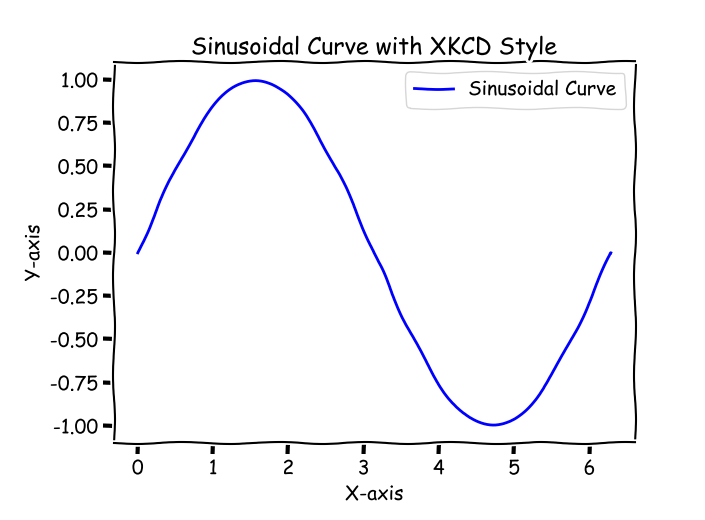
\includegraphics[width=\textwidth]{images/plot.png}
}
\newpage
